% Chapter Template

\chapter{Estat de l'art} % Main chapter title

\label{Chapter2} % Change X to a consecutive number; for referencing this chapter elsewhere, use \ref{ChapterX}

Per conèixer millor el potencial d'aquest mercat i saber les alternatives per a una major profunditat en el coneixement del sector, s'ha de realitzar un estudi del mercat existent per a comprovar la presència d'aplicacions que són similars, sigui per objectiu o per mercat, a \textit{Wisebite}. A continuació apareixen algunes de les aplicacions que s'han pogut trobar.
\\\\
El fet d'analitzar cadascuna d'elles et permet veure quines funcionalitats pots oferir al client perquè directament no existeix cap eina que les faciliti o bé per millorar les existents. S'ha volgut destacar sis plataformes similars a \textit{Wisebite}, algunes en millors aspectes que altres. En acabar de valorar cadascuna d'elles, es realitzarà un estudi ja més globalitzat que permeti veure quins avantatges ofereix \textit{Wisebite} al mercat actual.

%----------------------------------------------------------------------------------------
%	SECTION 1
%----------------------------------------------------------------------------------------

\section{Waiterio}

Aplicació\cite{waiterio} orientada especialment a substituir el \textit{TPV} d'un bar o restaurant. Disposa de funcionalitats com creació de menús i comandes, convidar companys de feina amb rols associats, visualització en mòbil i tauleta, reports periòdics i generació de factures totals o fraccionades.
\\\\
L'aplicació disposa d'entre unes 50.000 i 100.000 descàrregues al \textit{Play Store}. En general, conté moltes funcionalitats i té una interfície d'usuari ben cuidada que permet l'ús de l'aplicació de forma més còmode i confortable.
\\
\begin{figure}[H]
\centering
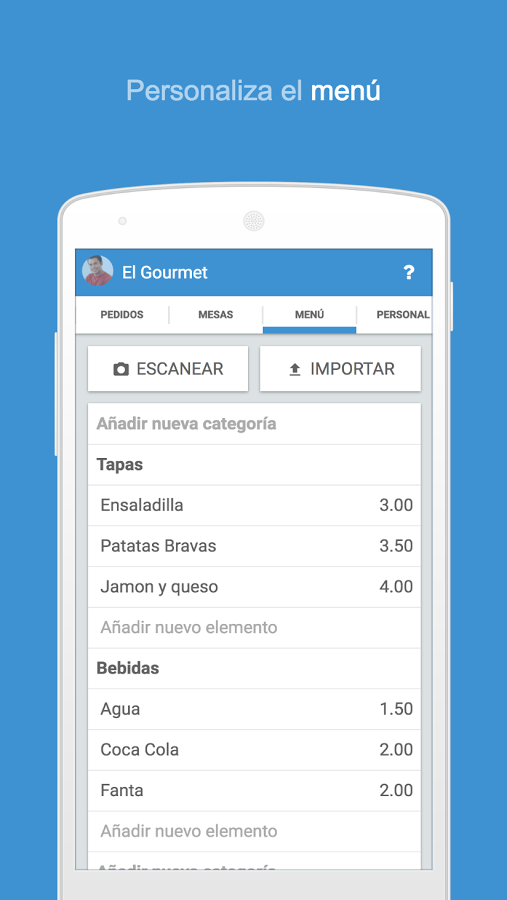
\includegraphics[scale=0.20]{Figures/waitero-1.png}
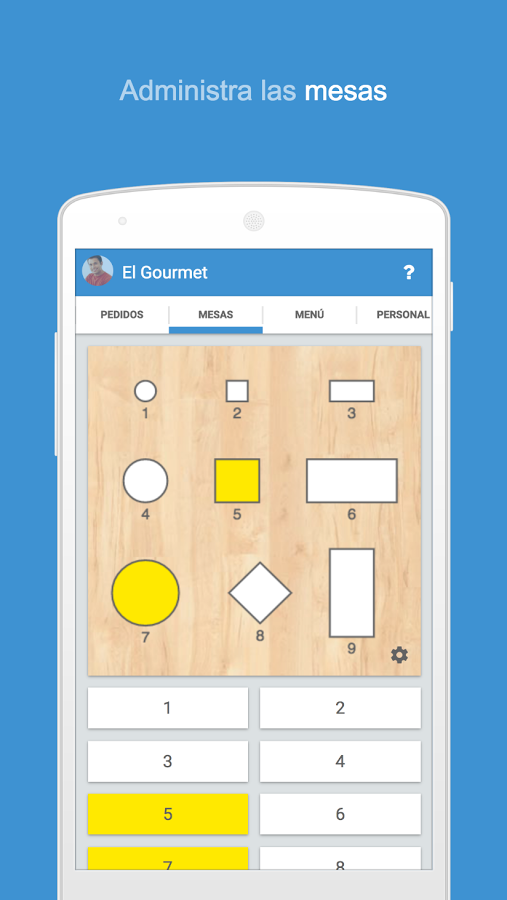
\includegraphics[scale=0.20]{Figures/waitero-2.png}
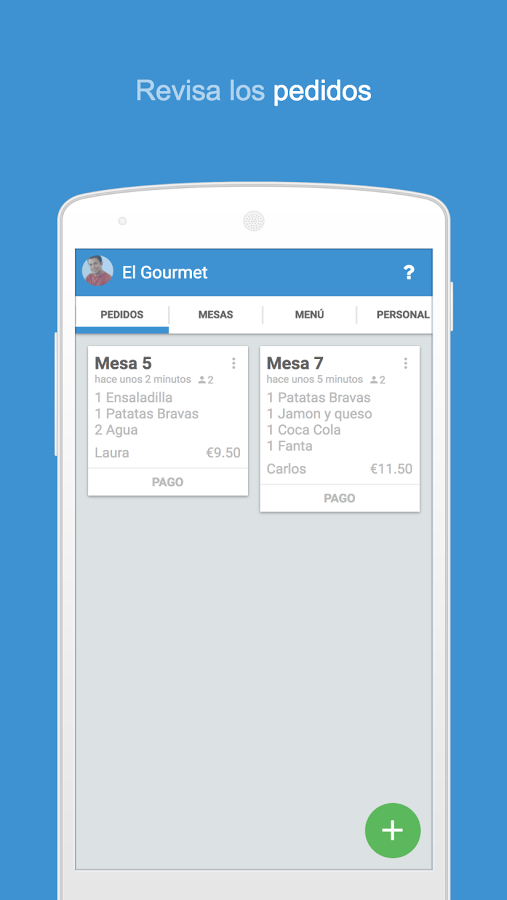
\includegraphics[scale=0.20]{Figures/waitero-3.png}
\caption{Captures de pantalla de Waitero}
\end{figure}



%----------------------------------------------------------------------------------------
%	SECTION 2
%----------------------------------------------------------------------------------------

\section{PrimeTray}

Aplicació\cite{primetray} orientada a les comandes del client a l'establiment. L'usuari té la capacitat de seleccionar un restaurant de la llista i fer la comanda en línia i anar-ho a buscar un cop és notificat. A més a més pot visualitzar l'estat en temps real de la seva comanda, és a dir, si està preparada o encara queda temps per poder-la rebre.
\\\\
L'aplicació té entre 500 i 1.000 descàrregues a la botiga d'aplicacions d'\textit{Android}. Tot i així té un 4.7 de valoració per part dels usuaris. En general l'aplicació està molt ben enfocada pel seu objectiu, és a dir, millorar la comoditat del client en els establiments de restauració als quals acudeix. Té una gestió de la interfície d'usuari prou bona que aconsegueix que sigui més fàcil utilitzar i familiaritzar-se amb l'aplicació. En contrapartida, les funcionalitats d'aquesta aplicació són bastants escasses. Fet que aconsegueix que perdi molts punts en comparació altres empreses.
\\
\begin{figure}[H]
\centering
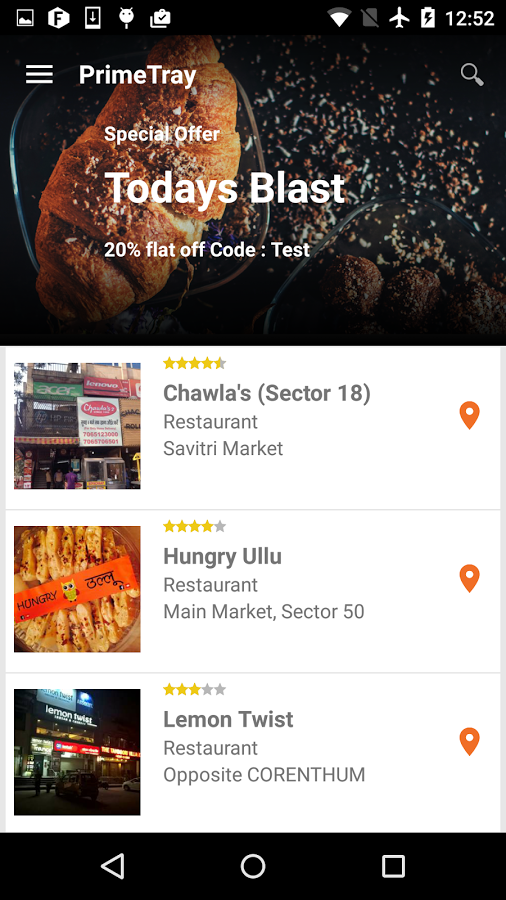
\includegraphics[scale=0.20]{Figures/primetray-1.png}
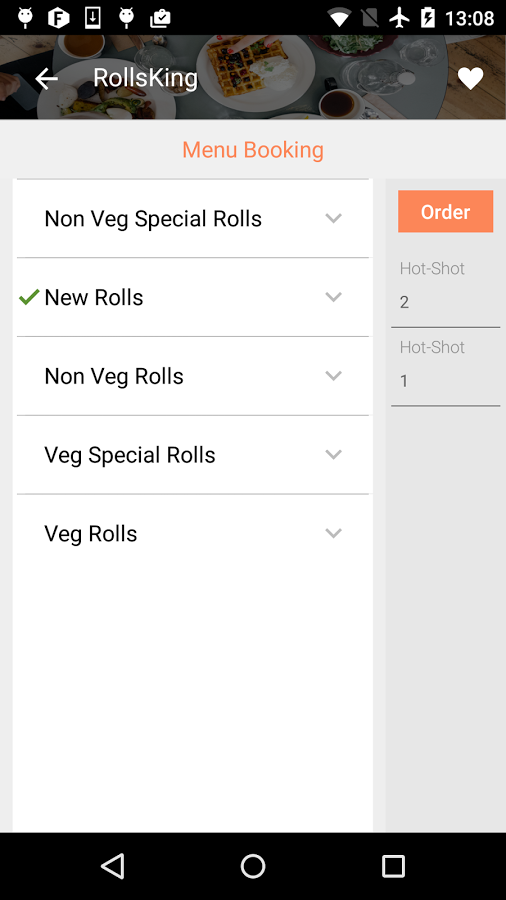
\includegraphics[scale=0.20]{Figures/primetray-2.png}
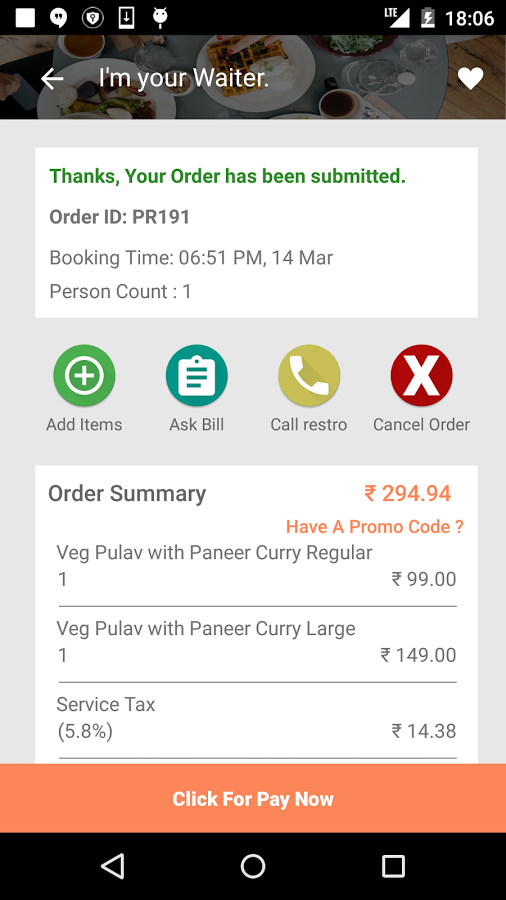
\includegraphics[scale=0.20]{Figures/primetray-3.png}
\caption{Captures de pantalla de PrimeTray}
\end{figure}

%----------------------------------------------------------------------------------------
%	SECTION 3
%----------------------------------------------------------------------------------------

\section{OrderSev}

Aplicació\cite{ordersev} orientada especialment a substituir el \textit{TPV} d'un bar o restaurant. Disposa de funcionalitats com creació de menús i comandes, generació de factures i vistes tant des de cuina com del cambrer. Gran punt a favor que disposa aquesta aplicació és la vista web de la qual disposa. Pots accedir de forma multiplataforma segons l'objectiu que tens amb l'aplicació.
\\\\
Disposa d'entre 500 i 1.000 descàrregues, i amb una nota mitjana de 5.0, però amb només 17 votacions, ha acabat sent una aplicació funcional però amb no gaire repercussió. El punt en contra que és que no li han dedicat el temps en la interfície d'usuari que comporta. Disposa d'unes vistes molt simples i molt poc estètiques.
\\\\
La gestió de la interfície d'usuari és quelcom molt important a l'hora de valorar una aplicació. Pel simple fet que els usuaris que la utilitzin no es fixaran en si l'algorisme i les tecnologies utilitzades són molt bones o no, sinó en quin aspecte té l'aplicació. És per això doncs que aquesta aplicació no ha acabat de triomfar, pel simple fet que la interfície no era l'adequada pel tipus d'usuari amb el qual treballava.
\\
\begin{figure}[H]
\centering
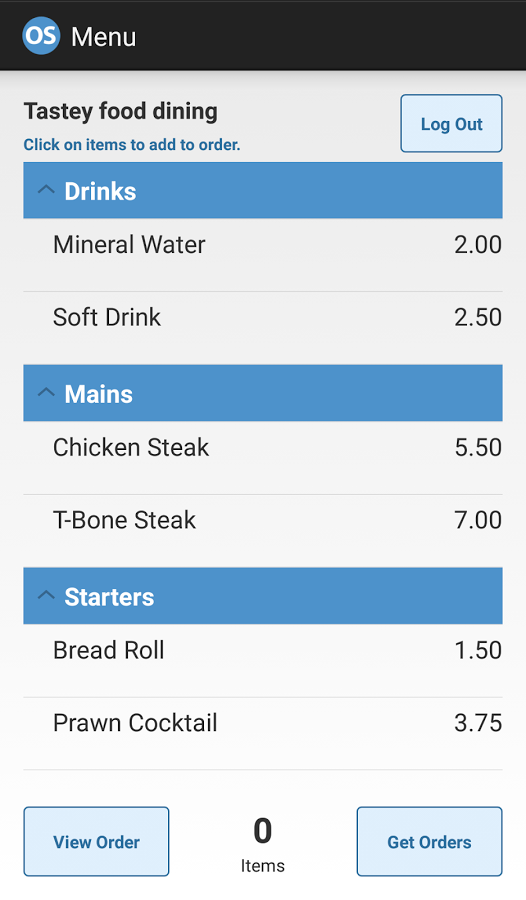
\includegraphics[scale=0.20]{Figures/ordersev-1.png}
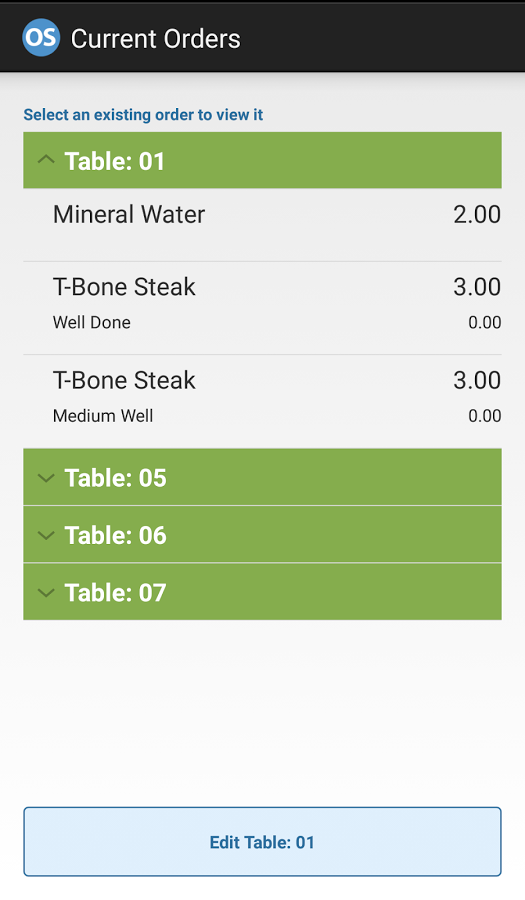
\includegraphics[scale=0.20]{Figures/ordersev-2.png}
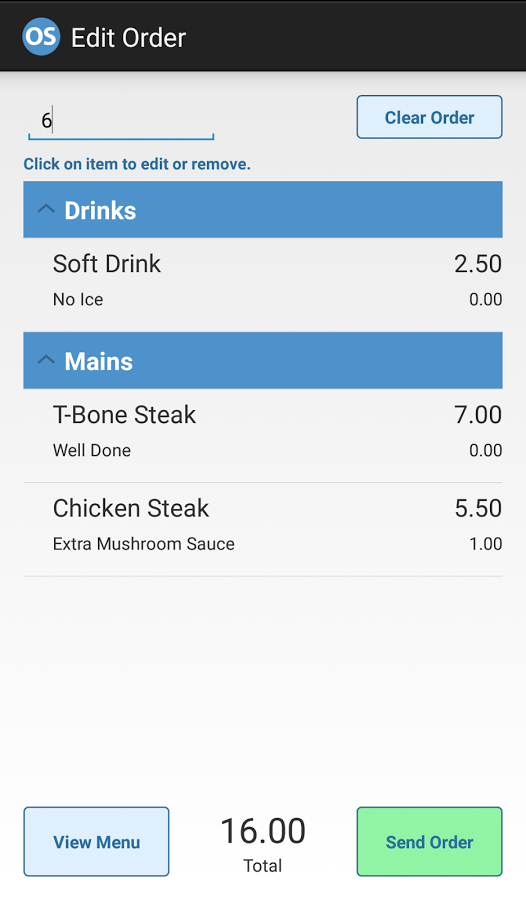
\includegraphics[scale=0.20]{Figures/ordersev-3.png}
\caption{Captures de pantalla de OrderSev}
\end{figure}

%----------------------------------------------------------------------------------------
%	SECTION 4
%----------------------------------------------------------------------------------------

\section{TabletWaiter}

Aplicació\cite{tabletwaiter} orientada a ser un estil de carta per a l'establiment. Cada taula d'un restaurant hauria d'haver-hi un dispositiu amb aquesta aplicació activa a on es pugui consultar els plats i seleccionar-los, així es rebria a cuina i ja podrien començar a preparar la comanda. També permet cridar al cambrer via aplicació i demanar el compte. Per altra banda, també disposa de la possibilitat que un cambrer la utilitzi per crear la comanda. És a dir, l'aplicació està preparada per ambdós perfils, ja sigui client com cambrer. Permet accedir-hi en la seva versió web, a on es pot crear els menús i parametritzar com vulguis el teu bar o restaurant.
\\\\
Aquesta aplicació, amb un conjunt de descàrregues situat entre 1.000 i 5.000 i un valor de 3.7 com a puntuació dels usuaris, es situa en un bon lloc en el mercat donat les funcionalitats que disposa. Tot i així, no ha acabat mai de despuntar a causa de la seva gestió de la interfície d'usuari. Les aplicacions per a dispositius mòbils han anat evolucionant en el que el seu disseny es refereix cap a un punt on totes les plataformes segueixen els mateixos patrons de disseny, patrons com \textit{Material Design}\cite{materialdesign}. Fet que no aplica aquesta aplicació. La plataforma disposa d'una interfície que no aplica cap tipus de patró de disseny, fet que dificulta la usabilitat de l'usuari.
\\
\begin{figure}[H]
\centering
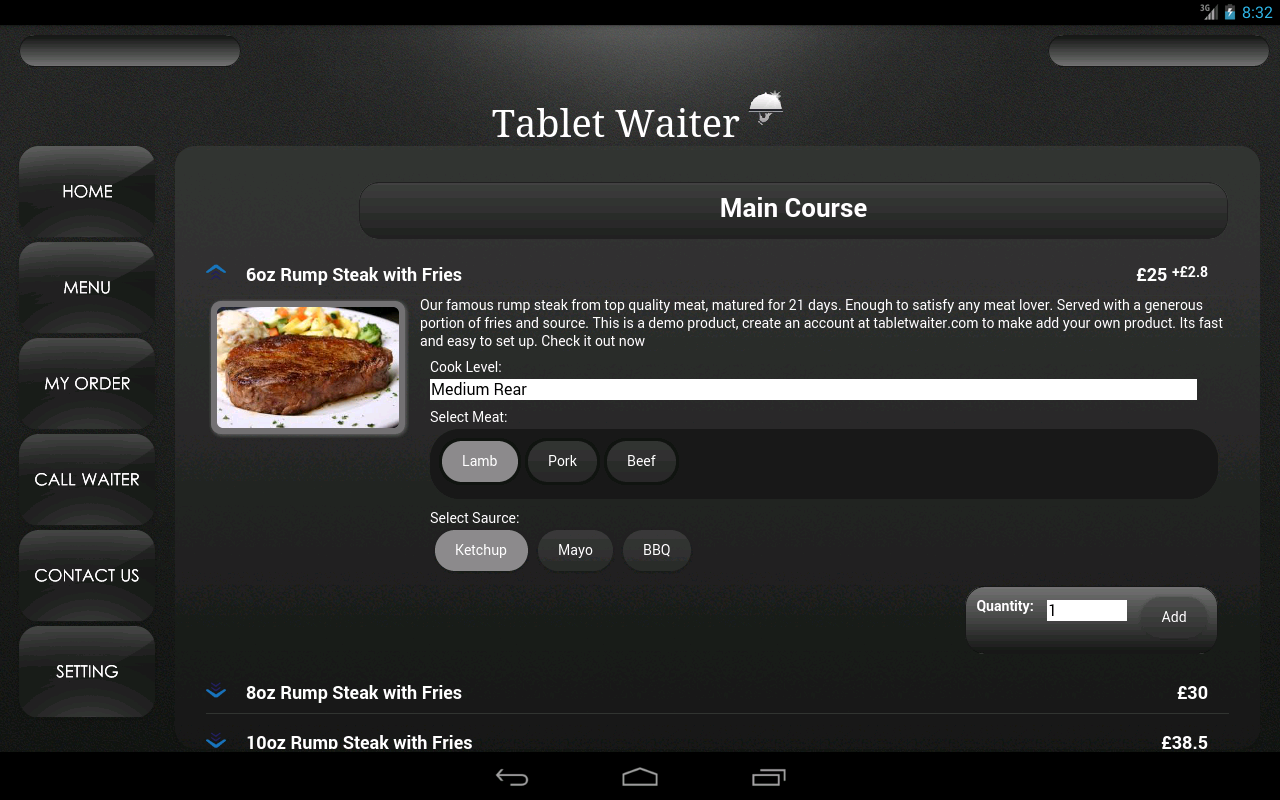
\includegraphics[scale=0.15]{Figures/tabletwaiter-1.png}
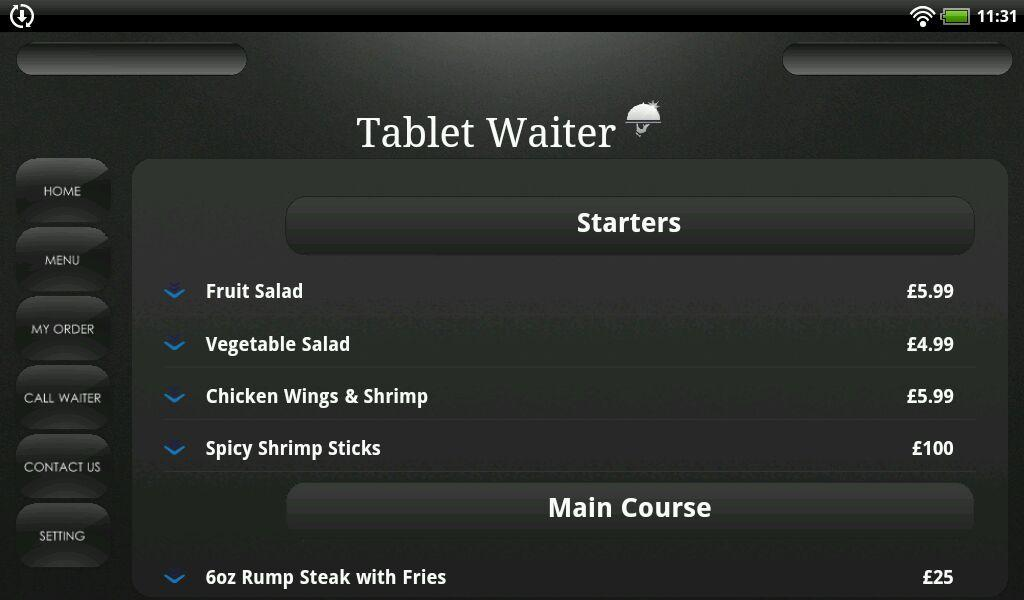
\includegraphics[scale=0.20]{Figures/tabletwaiter-2.png}
\caption{Captures de pantalla de TabletWaiter}
\end{figure}

%----------------------------------------------------------------------------------------
%	SECTION 5
%----------------------------------------------------------------------------------------

\newpage
\section{Cloud Waiter}

Aplicació\cite{cloudwaiter} orientada a les comandes del client a l'establiment. L'usuari té la capacitat d'escanejar un codi QR amb el qual podrà accedir a l'aplicació i realitzar la comanda. Així doncs l'usuari client que acudeix a l'establiment podrà estar-hi el temps que vegi precís i podrà demanar el que vulgui sense necessitat d'esperar al cambrer que l'assisteixi. A part, també disposa de la funcionalitat de poder cridar al cambrer perquè s'acosti a la taula tant per consultes com per demanar el compte.
\\\\
Plataforma amb un volum de descàrregues d'entre 1.000 i 5.000 i una valoració de 4.6 sobre 5 per part dels usuaris, es converteix en una aplicació bastant correcta en l'àmbit en el qual s'especialitza, és a dir, millorar l'experiència del client en l'establiment. Malauradament aquesta aplicació no ha acabat de sortir a la llum pel mateix problema que s'ha comentat en l'aplicació anterior, o sigui, la dolenta gestió d'interfície d'usuari.
\\
\begin{figure}[H]
\centering
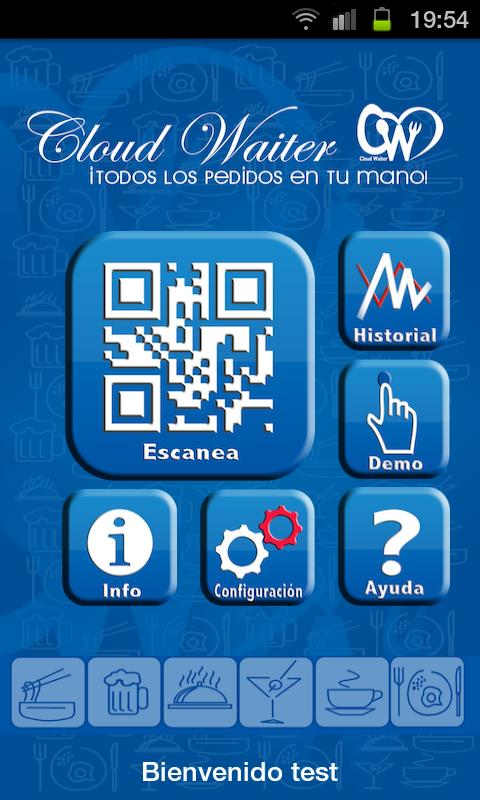
\includegraphics[scale=0.20]{Figures/cloudwaiter-1.jpg}
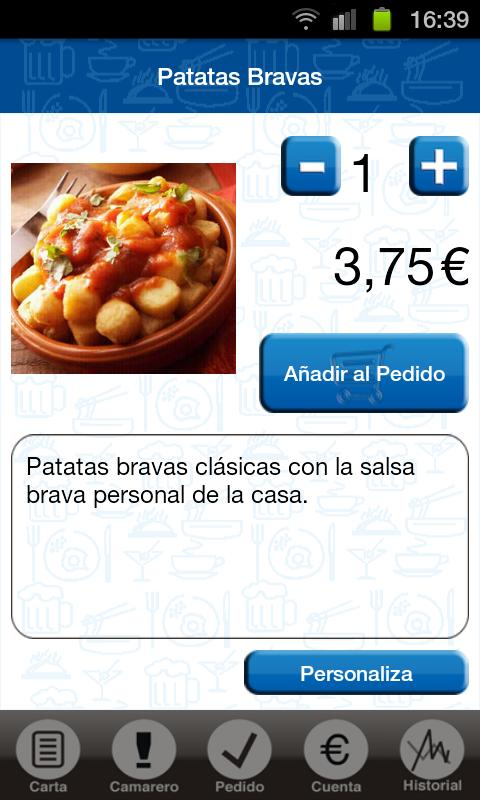
\includegraphics[scale=0.20]{Figures/cloudwaiter-2.jpg}
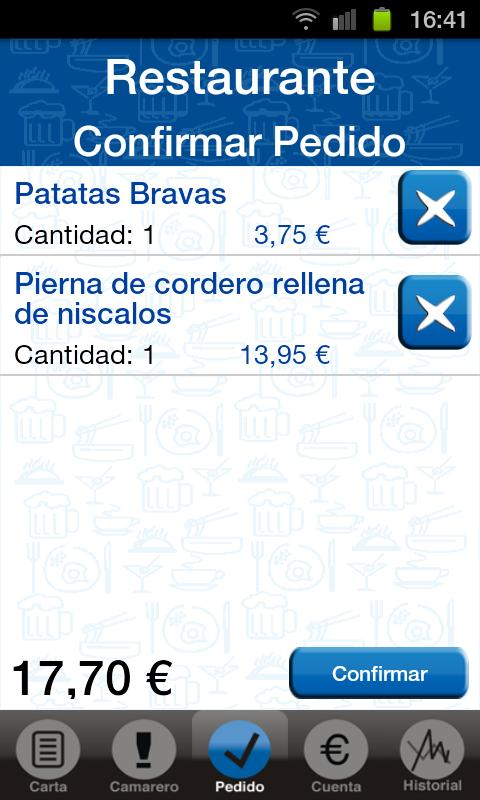
\includegraphics[scale=0.20]{Figures/cloudwaiter-3.jpg}
\caption{Captures de pantalla de OrderSev}
\end{figure}

%----------------------------------------------------------------------------------------
%	SECTION 6
%----------------------------------------------------------------------------------------

\section{FastOrder}

Aplicació\cite{fastorder} orientada a les comandes del client a l'establiment. L'usuari té la capacitat d'escanejar un codi QR amb el qual podrà accedir a l'aplicació i realitzar la comanda i tot el que sigui necessari. Diferents usuaris poden accedir a la mateixa comanda i modificar-la segons vegin convenient, fet que permet que cadascun dels clients d'una mateixa taula puguin fer la comanda de forma paral·lela.
\\\\
Aplicació amb més de 5.000 però amb menys de 10.000 descàrregues i amb una valoració de 4.7 per part de la comunitat d'usuaris, es situa amb una de les que disposa de més usuaris en comparació de les que s'han comparat. Aquesta plataforma disposa de funcionalitats un xic limitades en comparació de la competència, però en contrapartida té una interfície d'usuari molt ben cuidada. Fet que la permès situar-se amb el nombre de descàrregues que disposa actualment.
\\
\begin{figure}[H]
\centering
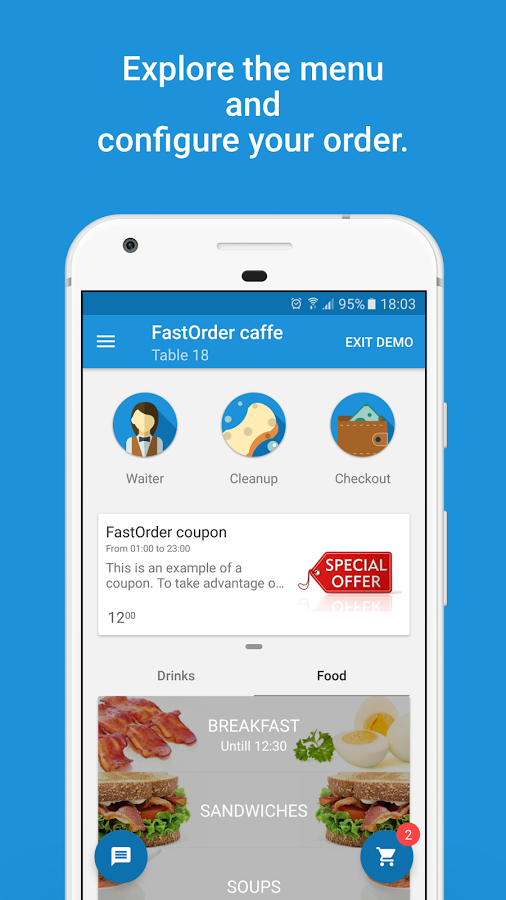
\includegraphics[scale=0.20]{Figures/fastorder-1.png}
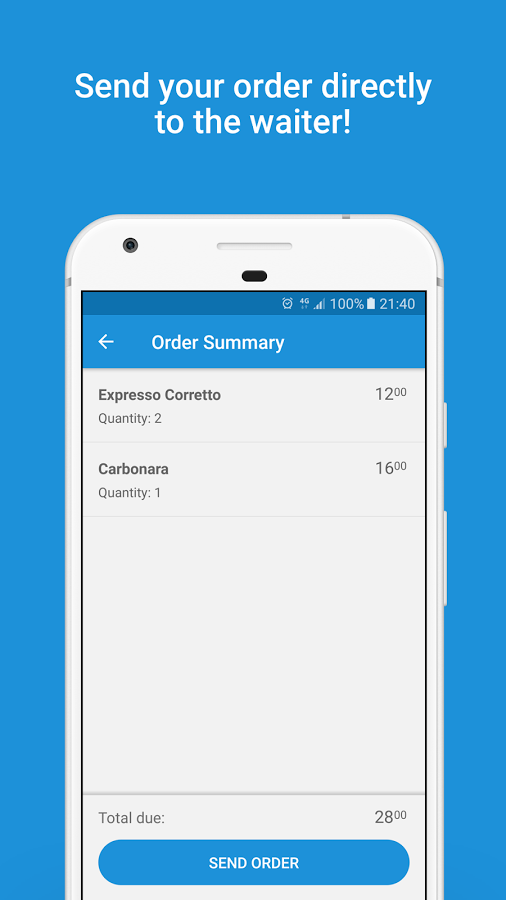
\includegraphics[scale=0.20]{Figures/fastorder-2.png}
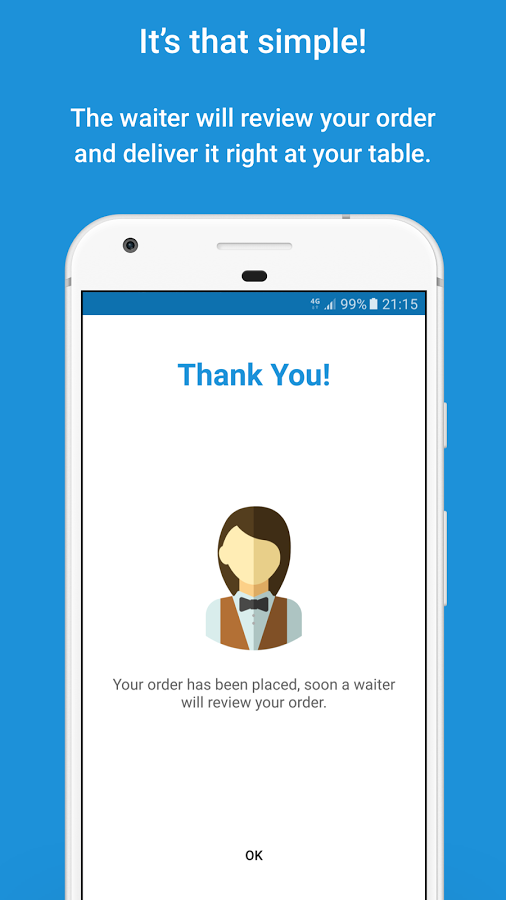
\includegraphics[scale=0.20]{Figures/fastorder-3.png}
\caption{Captures de pantalla de OrderSev}
\end{figure}

%----------------------------------------------------------------------------------------
%	SECTION 7
%----------------------------------------------------------------------------------------

\section{Conclusions}

Encara que hi ha moltes aplicacions relacionades amb aquest àmbit (si bé, amb objectius i funcionalitats molt diverses, en alguns casos molt dispars al projecte), s'ha fet una selecció prou representativa però tot i així reduïda, amb l'objectiu de realitzar una correcta anàlisi que permeti treure conclusions de forma còmoda i eficaç.
\\\\
Un cop realitzada aquesta selecció de potencials competidors de l'aplicació, i comprès (a grans trets) les seves funcionalitats i objectius, procedim a un estudi detallat comparant-ho amb la visió d'aquest projecte.
\\\\
El que s'ha pogut veure estudiant el mercat és que hi ha dos grans grups d'aplicacions. Per una banda, tenim els sistemes que només se centren en la gestió interna de l'establiment i poder realitzar comandes més fàcil i eficientment. Per altra banda, tenim les plataformes que permeten al client, que acudeix a l'establiment, viure una millor experiència i estar còmode en la seva estança. Resumint, hi ha aplicacions que milloren a l'empleat de l'establiment i altres que aporten comoditat al client.
\\\\
Altre punt realment important, i que s'ha pogut demostrar en l'anàlisi de cada una de les aplicacions anteriors, és la gestió de la interfície d'usuari (\textit{GUI}). Gran part dels usuaris que podrien arribar a utilitzar aquest tipus d'aplicacions o plataformes són usuaris no especialitzats en la tecnologia, també coneguts per l'anglicisme \textit{laypeople}. En conseqüència, és realment vital centrar-se a construir una bona experiència d'usuari i dissenyar una aplicació que sigui fàcil d'utilitzar, intuïtiva i fàcil d'aprendre per qualsevol tipus de perfil d'usuari. Un exemple podria ser \textit{FastOrder}, una aplicació que escasseja clarament de funcionalitats si ho comparem amb la resta d'aplicacions del mercat, però en canvi es situa la segona amb més descàrregues dins del \textit{Play Store}. Per què? Perquè al cap i a la fi el primer impacte que reps d'una aplicació, sigui mòbil o web, és la interfície d'aquesta. Si la plataforma disposa d'una bona experiència per l'usuari, aquest la seguirà utilitzant de forma genèrica i fins i tot l'acabarà recomanant al seu cercle.
\\\\
En conclusió, un cop estudiat quin és el mercat, es veu clar quina és la tendència i que pot aportar \textit{Wisebite} a aquest sector.
\\\\
Per un cantó, les nombroses funcionalitats que disposen les aplicacions comentades es podrien agrupar en tres grans grups: gestió de l'establiment, anàlisi de dades i relació amb el client. El primer d'ells es basa en tot el que engloba la digitalització de l'establiment, el segon és l'explotació de les dades digitalitzades per a la millora en l'eficiència i gestió del bar o el restaurant i per últim la millora en l'experiència del client en l'establiment. El fet és que no existeix cap plataforma que implanti les tres funcionalitats, com a molt dues d'elles. \textit{Wisebite} té la intenció d'adaptar les tres en una sola plataforma, i no només això, sinó millorar les prestacions de cada un d'elles.
\\\\
Per altra banda, i com ja s'ha comentat en estudiar cada un dels exemples anteriors, \textit{Wisebite} té molt a aportar en el que la gestió de la interfície d'usuari es tracta. No només es vol disposar d'un sistema òptim des d'un sentit computacional, sinó tenir una interfície d'usuari usable, intuïtiva i comprensible per qualsevol tipus de client, sobretot fent èmfasi en el sector \textit{laypeople}.
\\\\
Així doncs, \textit{Wisebite} aportarà un nou estil d'aplicació desconegut en el sector fins al dia d'avui que facilitarà el dia a dia a tota persona relacionada, ja sigui client com empleat.